\subsection{Model}

\begin{figure}[H]
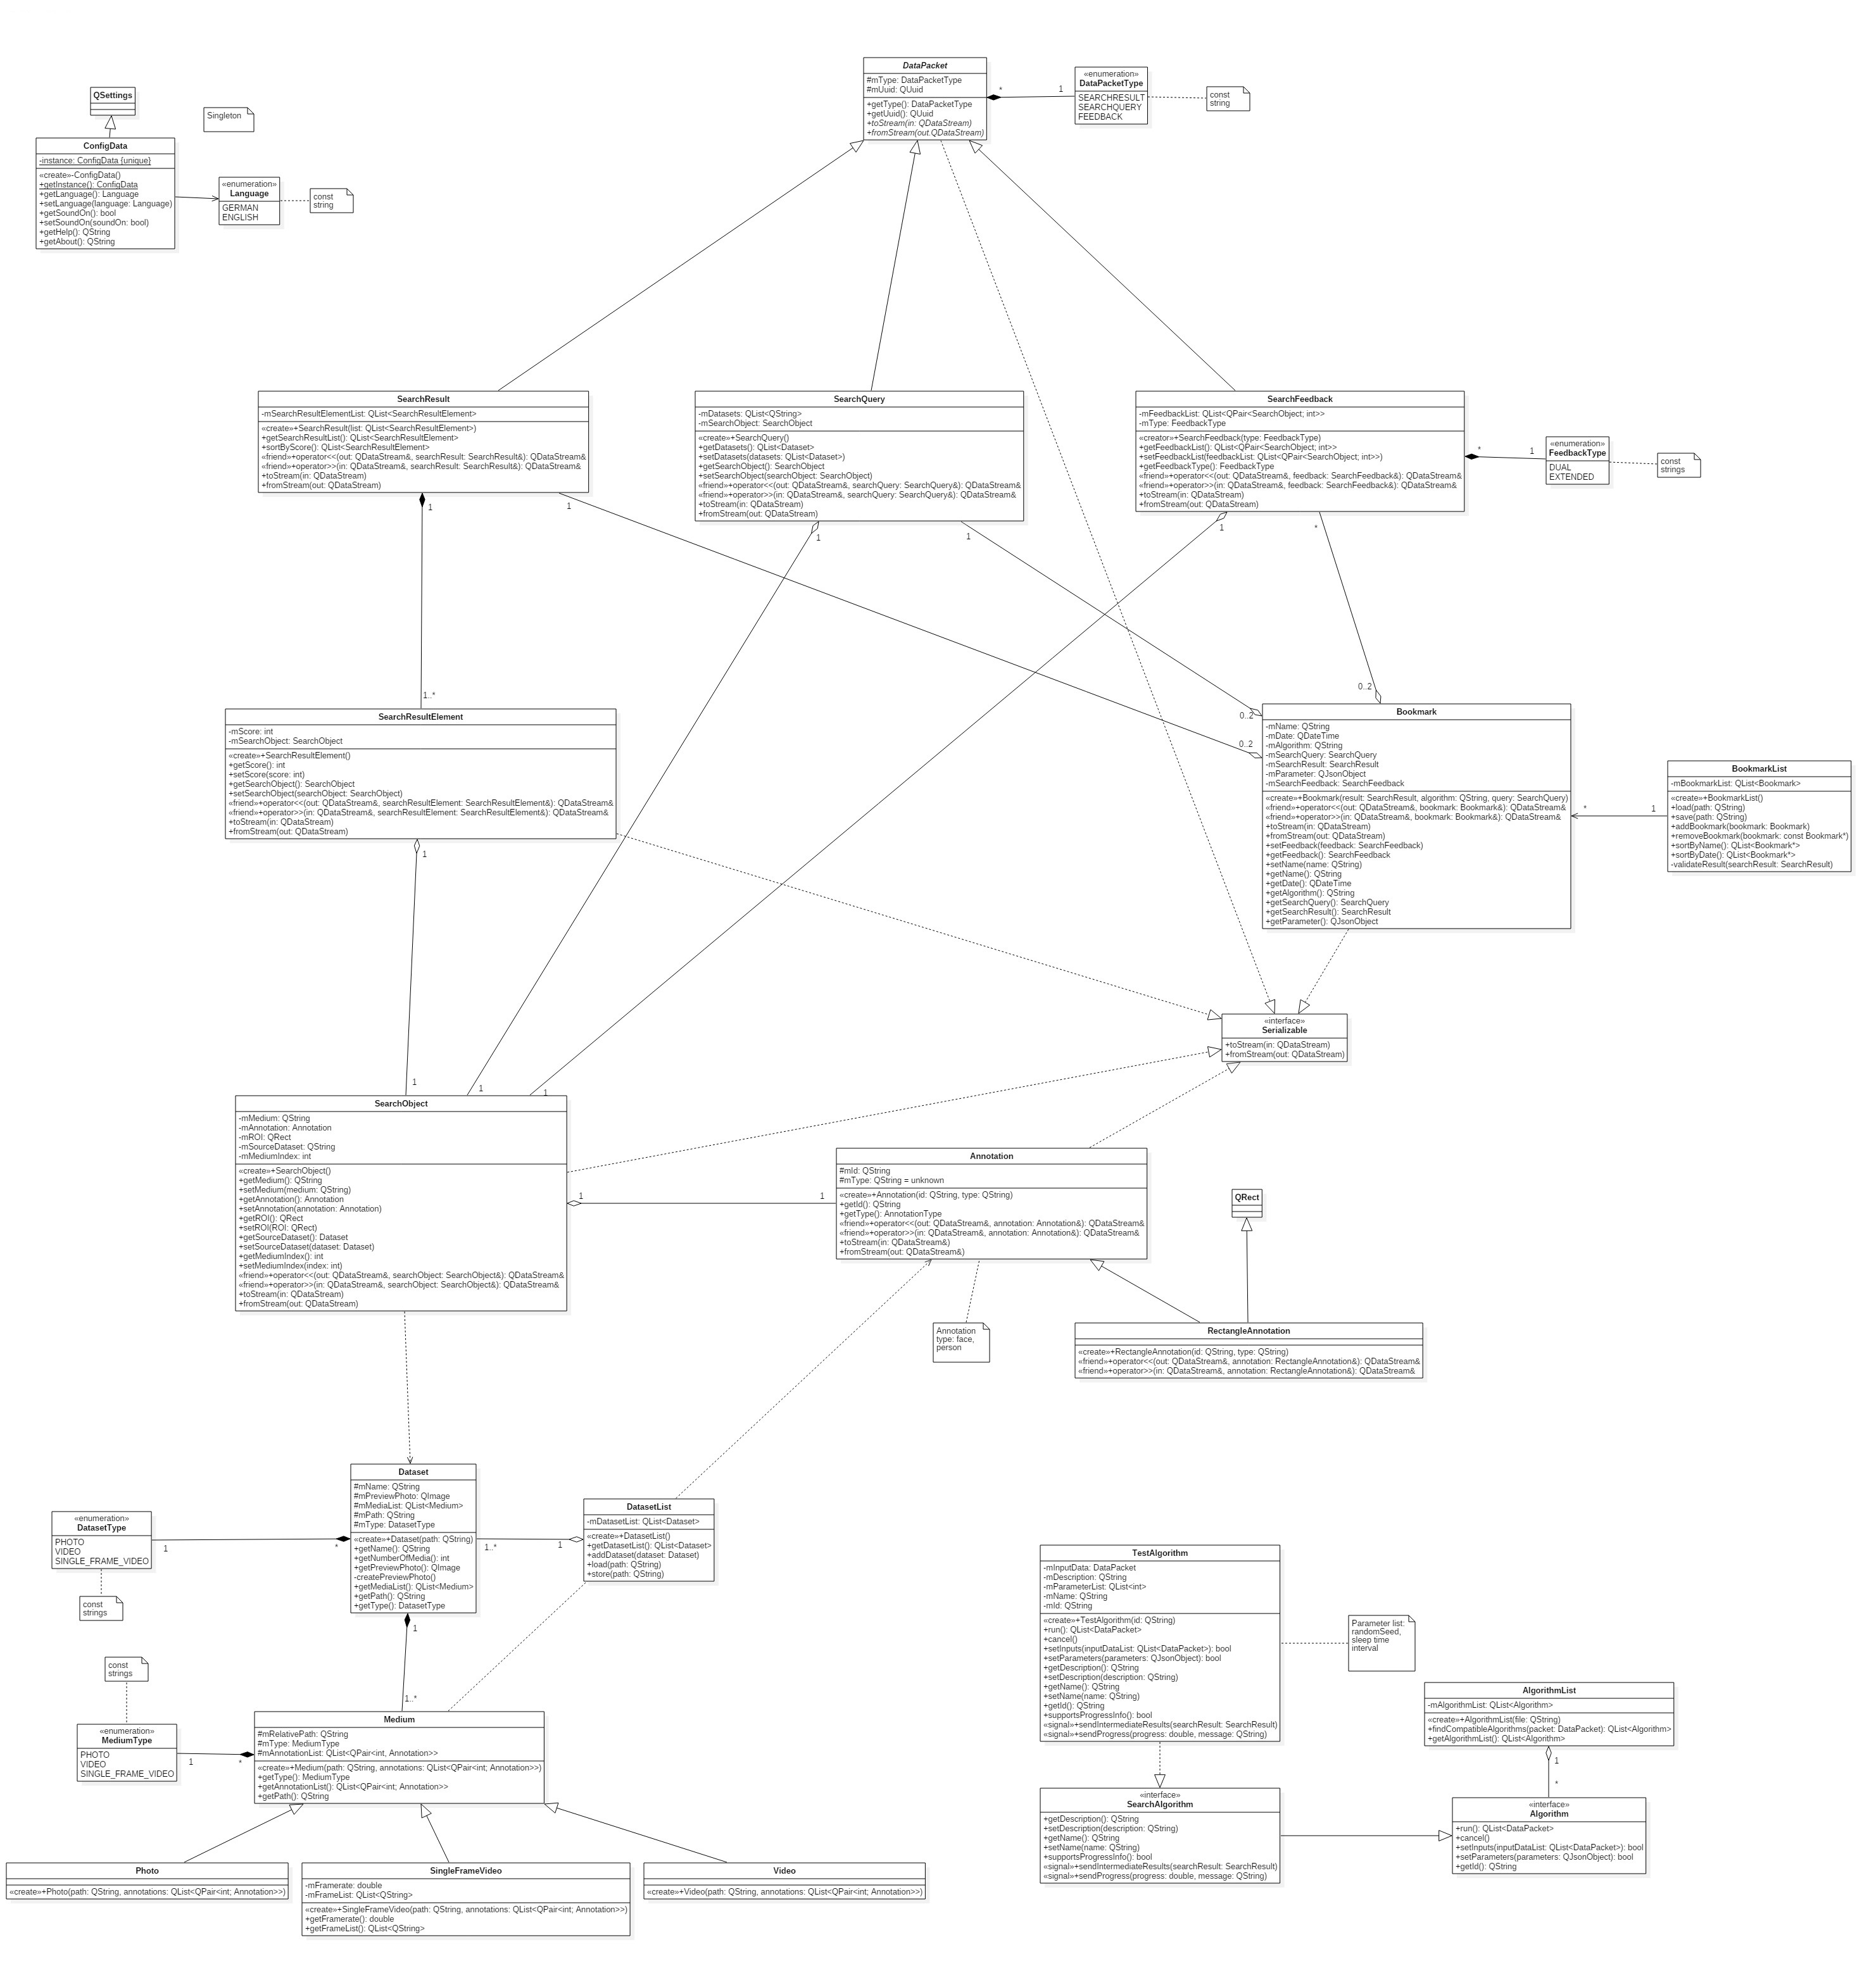
\includegraphics[width=1\linewidth]{img/Klassendiagramm/Model}
\caption{Model}
\label{fig:model}
\end{figure}


\subsection*{ConfigData}

Die Klasse ConfigData speichert die Benutzereinstellungen Sprache und Benachrichtigungston. Außerdem werden die Hilfe- und Aboutdateien gelesen.

\begin{figure}[H]
\centering
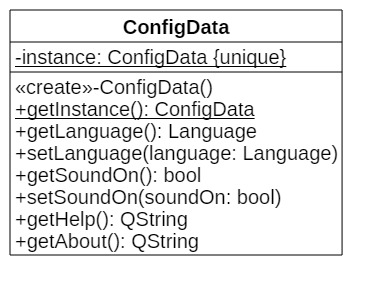
\includegraphics[scale=0.5]{img/Klassendiagramm/Klassen/ConfigData}
\label{fig:configData}
\end{figure}

Attribute
\begin{itemize}
\item\textit{private ConfigData instance} Die einzige Instanz von ConfigData. 
\end{itemize}

Methoden
\begin{itemize}
\item \textit{private ConfigData()} Erzeugt ein neues ConfigData Objekt.
\item \textit{public ConfigData getInstance()} Liefert die ConfigData Instanz zurück. Dies stellt sicher, dass nur eine Instanz von ConfigData existiert.
\item \textit{public Language getLanguage()} Lädt die vom Benutzer gewählte Sprache.
\item \textit{public void setLanguage(Language language)} Speichert die vom Benutzer gewählte Sprache.
\item \textit{public bool getSoundOn()} Lädt die vom Benutzer gewählte Toneinstellung.
\item \textit{public void setSoundOn(bool soundOn)} Speichert die vom Benutzer gewählte Toneinstellung.
\item \textit{public QString getHelp()} Lädt die Hilfedatei und gibt deren Inhalt zurück.
\item \textit{public QString getAbout()} Lädt die Aboutdatei und gibt deren Inhalt zurück.
\end{itemize}

\subsection*{<<enumeration>> Language}
Language repräsentiert die verfügbaren Sprachen: Deutsch und Englisch.

\begin{figure}[H]
\centering
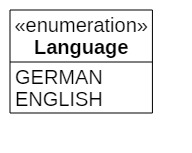
\includegraphics[scale=0.5]{img/Klassendiagramm/Klassen/Language}
\label{fig:language}
\end{figure}

\subsection*{Annotation : public Serializable}
Eine Annotation ist ein in den Datensätzen vordefinierter Bereich eines Bildes oder Videos, der den Typ Face oder Person haben kann.

\begin{figure}[H]
\centering
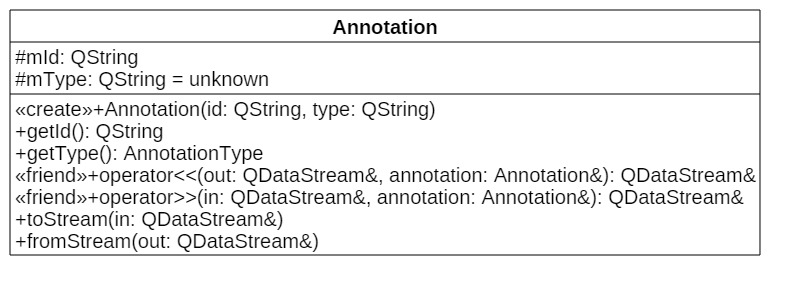
\includegraphics[scale=0.5]{img/Klassendiagramm/Klassen/Annotation}
\label{fig:annotation}
\end{figure}

Attribute
\begin{itemize}
\item\textit{protected QString mId} Diese Id identifiziert diese Annotation in einem  Medium.
\item\textit{protected QString mType} Beschreibt den Typ dieser Annotation.
\end{itemize}

Methoden
\begin{itemize}
\item \textit{public Annotation(QString Id)} Gibt eine Instanz dieser Klasse zurück. Die übergebene Id identifiziert die Annotation in einem Medium.
\item \textit{public QString getId()} Gibt die Id der Annotation zurück.
\item \textit{public AnnotationType getType()} Gibt den Typ der Annotation zurück.
\item \textit{public friend QDataStream\& operator<<(QDataStream\& out, Annotation\& annotation)} Speichert die Annotation in einer Datei.
\item \textit{public friend QDataStream\& operator>>(QDataStream\& in, Annotation\& annotation)} Lädt die Annotation aus einer Datei.
\item \textit{public void toStream(QDataStream in)} Speichert die Annotation, durch den Aufruf von operator<<, in einer Datei.
\item \textit{public void fromStream(QDataStream out)} Lädt die Annotation, durch den Aufruf von operator>>, aus einer Datei.
\end{itemize}

\subsection*{RectangleAnnotation : public Annotation, public QRect}
Eine rechteckige Annotation.

\begin{figure}[H]
\centering
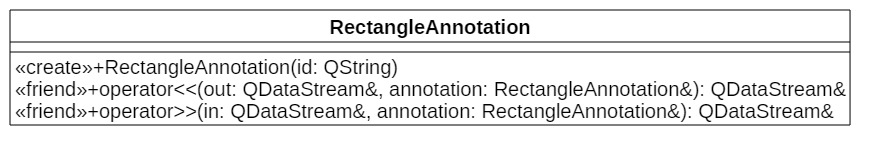
\includegraphics[scale=0.5]{img/Klassendiagramm/Klassen/RectangleAnnotation}
\label{fig:rectangleAnnotation}
\end{figure}

Methoden
\begin{itemize}
\item \textit{public RectangleAnnotation(QString id)} Erzeugt ein Objekt von RectangleAnnotation. Die übergebene Id Identifiziert die Annotation in einem Medium.
\item \textit{public friend QDataStream\& operator<<(QDataStream\& out, RectangleAnnotation\& annotation)} Speichert die RectangleAnnotation in einer Datei.
\item \textit{public friend QDataStream\& operator>>(QDataStream\& in, RectangleAnnotation\& annotation)} Lädt die RectangleAnnotation aus einer Datei.
\end{itemize}

\subsection*{DataPacket : public Serializable}
Ein DataPacket ist eine Eingabe für den Algorithmus.

\begin{figure}[H]
\centering
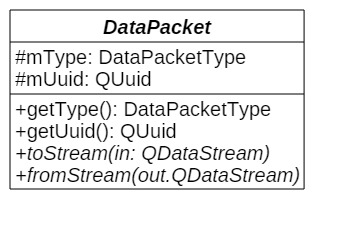
\includegraphics[scale=0.5]{img/Klassendiagramm/Klassen/DataPacket}
\label{fig:dataPacket}
\end{figure}

Attribute
\begin{itemize}
\item\textit{protected DataPacketType mType} Beschreibt den Typ dieses DataPackets.
\item\textit{protected QUuid mUuid} Identifiziert dieses DataPacket eindeutig. 
\end{itemize}

Methoden
\begin{itemize}
\item \textit{public DataPacketType getType()} Gibt den Typ des DataPackets zurück, abhängig von der Kindklasse.
\item\textit{public QUuid getUuid} Gibt die eindeutige Id dieses DataPacktets zurück.
\item \textit{public abstract void toStream(QDataStream in)} Speichert das DataPacket, durch den Aufruf von operator<<, in einer Datei.
\item \textit{public abstract void fromStream(QDataStream out)} Speichert das DataPacket, durch den Aufruf von operator>>, in einer Datei.
\end{itemize}

\subsection*{<<enumeration>> DataPacketType}
DataPacketType enthält die Typen von DataPackets, also die vorhandenen Kindklassen.

\begin{figure}[H]
\centering
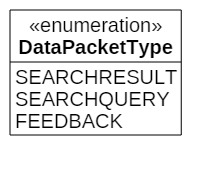
\includegraphics[scale=0.5]{img/Klassendiagramm/Klassen/DataPacketType}
\label{fig:dataPacketType}
\end{figure}

\subsection*{SearchQuery : DataPacket}
Eine SearchQuery ist eine Suchanfrage an den Algorithmus.

\begin{figure}[H]
\centering
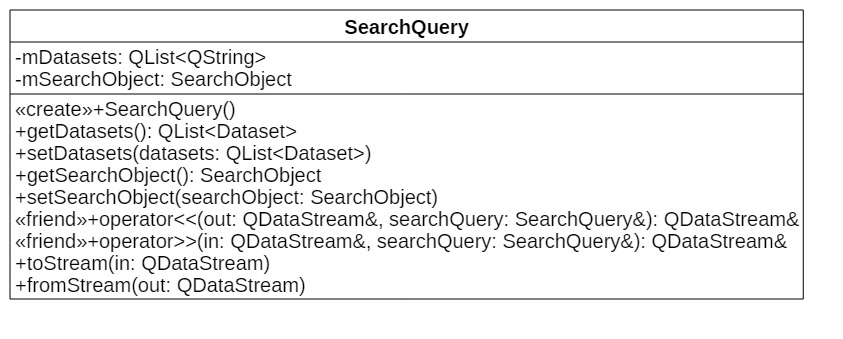
\includegraphics[scale=0.5]{img/Klassendiagramm/Klassen/SearchQuery}
\label{fig:searchQuery}
\end{figure}

Attribute
\begin{itemize}
\item\textit{private QList<QString> mDatasets} Beschreibt den Suchraum der Suchanfrage.
\item\textit{private SearchObject mSearchObject} Das zu dieser Suchanfrage gehörende SearchObject.
\end{itemize}

Methoden
\begin{itemize}
\item \textit{public SearchQuery()} Erzeugt ein SearchQuery-Objekt.
\item \textit{public QList<Dataset> getDatasets()} Gibt den Suchraum, in Form von einer Datensatzliste, zurück.
\item \textit{public void setDatasets(QList<Dataset> datasets)} Setzt den Suchraum für die Suchanfrage.
\item \textit{public SearchObject getSearchObject()} Gibt das SearchObject für diese Anfrage zurück.
\item \textit{public void setSearchObject(SearchObject searchObject)} Setzt das SearchObject für diese Anfrage.
\item \textit{public friend QDataStream\& operator<<(QDataStream\& out, SearchQuery\& searchQuery)} Speichert die SearchQuery in einer Datei.
\item \textit{public friend QDataStream\& operator>>(QDataStream\& in, SearchQuery\& searchQuery)} Lädt die SearchQuery aus einer Datei.
\item \textit{public void toStream(QDataStream in)} Speichert die SearchQuery, durch den Aufruf von operator<<, in einer Datei.
\item \textit{public void fromStream(QDataStream out)} Lädt die SearchQuery, durch den Aufruf von operator>>, aus einer Datei.
\end{itemize}

\subsection*{SearchResult : DataPacket}
Ein SearchResult ist die Ausgabe eines Algorithmus. Allerdings kann es auch eine Eingabe sein, wenn ein Algorithmus auf einem bestehenden Suchergebnis weiterarbeitet.

\begin{figure}[H]
\centering
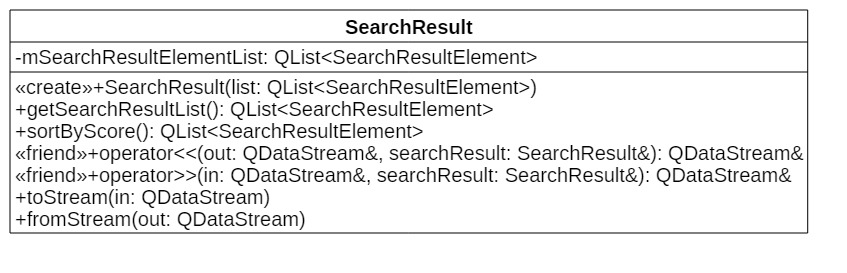
\includegraphics[scale=0.5]{img/Klassendiagramm/Klassen/SearchResult}
\label{fig:searchResult}
\end{figure}

Attribute
\begin{itemize}
\item\textit{private QList<SearchResultElement> mSearchResultElementList} Die Liste der zu diesem SearchResult gehörenden SearchResultElements.
\end{itemize}

Methoden
\begin{itemize}
\item \textit{public SearchResult(QList<SearchResultElement> list)} Erzeugt ein neues SearchResult, das eine Liste von SearchResultElements enthält.
\item \textit{public QList<SearchResultElement> getSearchResultList()} Gibt die Liste der SearchResultElements zurück.
\item \textit{public void sortByScore()} Sortiert die Ergebnisliste nach dem Score.
\item \textit{public friend QDataStream\& operator<<(QDataStream\& out, SearchResult\& searchResult)} Speichert das SearchResult in einer Datei.
\item \textit{public friend QDataStream\& operator>>(QDataStream\& in, SearchResult\& searchResult)} Lädt das SearchResult aus einer Datei.
\item \textit{public void toStream(QDataStream in)} Speichert das SearchResult, durch den Aufruf von operator<<, in einer Datei.
\item \textit{public void fromStream(QDataStream out)} Lädt das SearchResult, durch den Aufruf von operator>>, aus einer Datei.
\end{itemize}

\subsubsection*{SearchResultElement : public Serializable}
Ein SearchResultElement ist ein Element von SearchResult. Abgesehen von einem SearchObject enthält es einen Score für dieses, der durch den Algorithmus bestimmt und gesetzt wurde.

\begin{figure}[H]
\centering
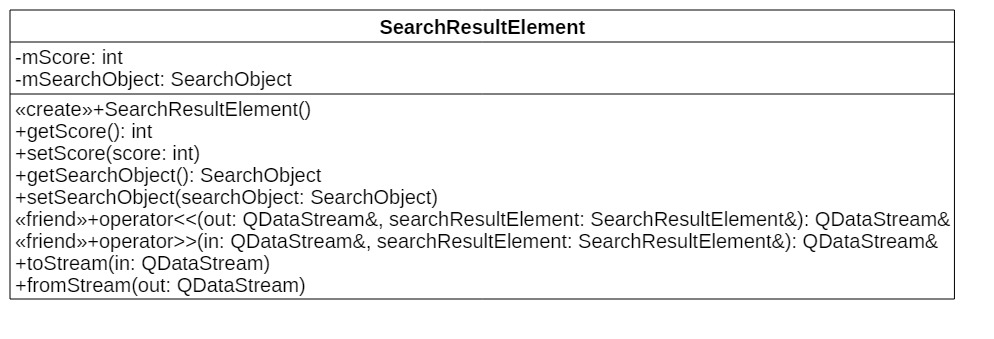
\includegraphics[scale=0.5]{img/Klassendiagramm/Klassen/SearchResultElement}
\label{fig:searchResultElement}
\end{figure}

Attribute
\begin{itemize}
\item\textit{private int mScore} Vom Suchalgorithmus zugewiesene Zahl, die die Übereinstimmung dieses SearchResultElements mit dem SearchObject der SearchQuery beschreibt.
\item\textit{private SearchObject mSearchObject} Das zu diesem SearchResultElement gehörende SearchObject.
\end{itemize}

Methoden
\begin{itemize}
\item \textit{public SearchResultElement()} Erzeugt ein SearchResultElement.
\item \textit{public int getScore()} Gibt den Score für dieses Element zurück.
\item \textit{public void setScore(int score)} Setzt den Score für dieses Element.
\item \textit{public SearchObject getSearchObject()} Gibt das SearchObject zurück.
\item \textit{public void setSearchObject(SearchObject searchObject)} Setzt das übergebene SearchObject für das Element.
\item \textit{public friend QDataStream\& operator<<(QDataStream\& out, SearchResultElement\& searchResultElement)} Speichert das SearchResultElement in einer Datei.
\item \textit{public friend QDataStream\& operator>>(QDataStream\& in, SearchResultElement\& searchResultElement)} Lädt das SearchResultElemnt aus einer Datei.
\item \textit{public void toStream(QDataStream in)} Speichert das SearchResultElement, durch den Aufruf von operator<<, in einer Datei.
\item \textit{public void fromStream(QDataStream out)} Lädt das SearchResultElement, durch den Aufruf von operator>>, aus einer Datei.
\end{itemize}

\subsection*{SearchObject : public Serializable}
Das SearchObject repräsentiert eine Annotation oder ein Rechteck in einem Bild oder Frame eines Videos aus einem Datensatz.

\begin{figure}[H]
\centering
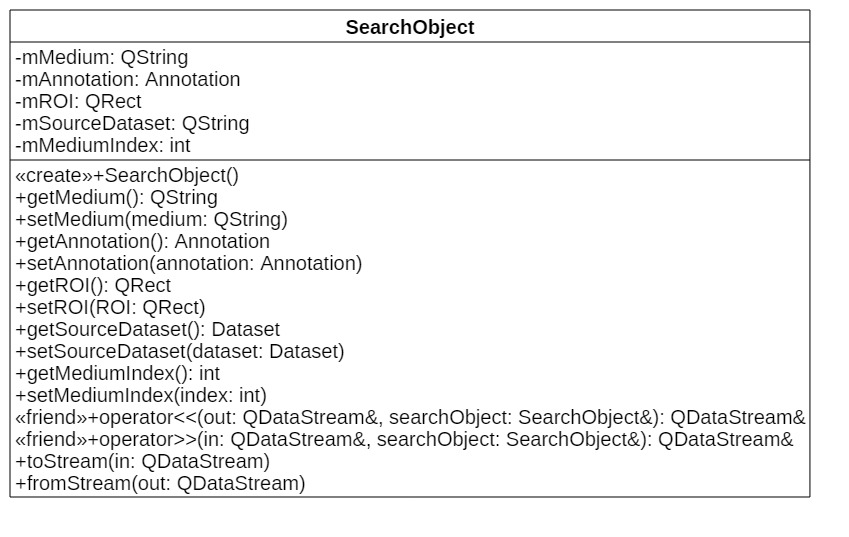
\includegraphics[scale=0.5]{img/Klassendiagramm/Klassen/SearchObject}
\label{fig:searchObject}
\end{figure}

Attribute
\begin{itemize}
\item\textit{private QString mMedium} Der Pfad des zugehörigen Mediums.
\item\textit{private Annotation mAnnotation} Die ausgewählte Annotation.
\item\textit{private QRect mROI} Die \enquote{region of interest} im zugehörigem Medium.
\item\textit{private QString mSourceDataset} Der Pfad des Datensatzes, in dem sich das Medium befindet.
\item\textit{private int mMediumIndex} Beschreibt die Framenummer des Mediums in einem Video.
\end{itemize}

Methoden
\begin{itemize}
\item \textit{public SearchObject} Erzeugt ein SearchObject.
\item \textit{public QString getMedium()} Gibt den Dateipfad des Mediums zurück.
\item \textit{public void setMedium(QString medium)} Setzt das Medium auf den gegebenen Dateipfad, relativ zum SourceDataset.
\item \textit{public Annotation getAnnotation()} Gibt die Annotation im Medium zurück.
\item \textit{public void setAnnotation(Annotation annotation)} Setzt eine Annotation eines Mediums für das SearchObject.
\item \textit{public QRect getROI()} Gibt ein QRect zurück, das die \enquote{region of interest} im Medium repräsentiert.
\item \textit{public void setROI(QRect ROI)} Setzt ein QRect als ROI.
\item \textit{public Dataset getSourceDataset} Gibt den Datensatz, in dem sich das Medium befindet zurück.
\item \textit{public void setSourceDataset(Dataset dataset)} Setzt den Datensatz, in dem sich das Medium befindet.
\item \textit{public int getMediumIndex()} Gibt den Index eines Mediums, also den Frame in einem Video zurück.
\item \textit{public void setMediumIndex(int index)} Setzt den MediumIndex.
\item \textit{public friend QDataStream\& operator<<(QDataStream\& out, SearchObject\& searchObject)} Speichert das SearchObject in einer Datei.
\item \textit{public friend QDataStream\& operator>>(QDataStream\& in, SearchObject\& searchObject)} Lädt das SearchObject aus einer Datei.
\item \textit{public void toStream(QDataStream in)} Speichert das SearchObject, durch den Aufruf von operator<<, in einer Datei.
\item \textit{public void fromStream(QDataStream out)} Lädt das SearchObject, durch den Aufruf von operator>>, aus einer Datei.
\end{itemize}

\subsection*{SearchFeedback : DataPacket}
Das SearchFeedback gibt an, wie gut das vom Algorithmus erzeugte Suchergebnis ist.

\begin{figure}[H]
\centering
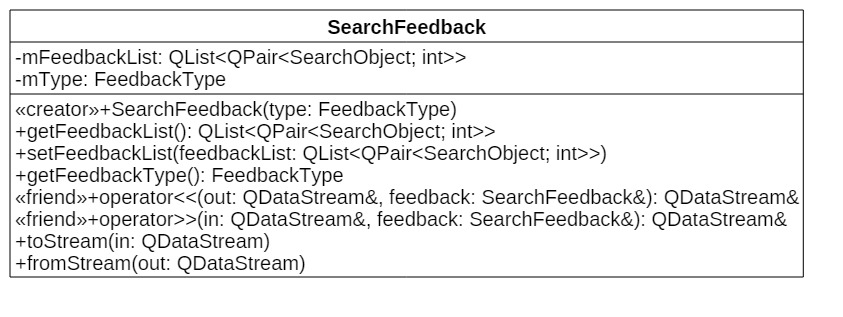
\includegraphics[scale=0.5]{img/Klassendiagramm/Klassen/SearchFeedback}
\label{fig:searchFeedback}
\end{figure}

Attribute
\begin{itemize}
\item\textit{private QList<QPair<SearchObject, int>>} Der Integer-Wert beschreibt das zum SearchObject gehörende Feedback.
\item\textit{private FeedbackType mType} Der Typ des Feedbacks, entweder dual oder extended.
\end{itemize}

Methoden
\begin{itemize}
\item \textit{public SearchFeedback(FeedbackType type)} Erzeugt ein neues SearchFeedback Objekt. Der Typ kann entweder dual oder extended sein.
\item \textit{public QList<QPair<SearchObject, int>>  getFeedbackList()} Gibt die FeedbackList  zurück.
\item \textit{public void setFeedbackList(QList<QPair<SearchObject, int>> feedbackList)} Setzt die FeedbackList auf die übergebene Liste.
\item \textit{public FeedbackType getFeedbackType()} Gibt den Feedback-Typ zurück.
\item \textit{public friend QDataStream\& operator<<(QDataStream\& out, Feedback\& feedback)} Speichert das Feedback in einer Datei.
\item \textit{public friend QDataStream\& operator>>(QDataStream\& in, Feedback\& feedback)} Lädt das Feedback aus einer Datei.
\item \textit{public void toStream(QDataStream in)} Speichert das Feedback, durch den Aufruf von operator<<, in einer Datei.
\item \textit{public void fromStream(QDataStream out)} Lädt das Feedback, durch den Aufruf von operator>>, aus einer Datei.
\end{itemize} 

\subsubsection*{<<enumeration>> FeedbackType}
Der FeedbackType kann dual (positiv, negativ, neutral) oder extended (Werte von 1 bis 10) sein.

\begin{figure}[H]
\centering
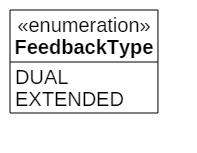
\includegraphics[scale=0.5]{img/Klassendiagramm/Klassen/FeedbackType}
\label{fig:feedbackType}
\end{figure}

\subsection*{<<interface>> Serializable}
Das Interface Serializable ist dazu da, damit die implementierenden Klassen serialisierbar sind.

\begin{figure}[H]
\centering
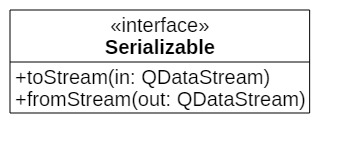
\includegraphics[scale=0.5]{img/Klassendiagramm/Klassen/Serializable}
\label{fig:serializable}
\end{figure}

Methoden
\begin{itemize}
\item \textit{public void toStream(QDataStream in)} Speichert das serialisierbare Objekt in einer Datei.
\item \textit{public void fromStream(QDataStream out)} Lädt das serialisierbare Objekt aus einer Datei.
\end{itemize}

\subsection*{Bookmark : public Serializable}
Ein Bookmark speichert ein Suchergebnis, eine Suchanfrage und das Feedback, sodass ein früherer Suchvorgang wiederhergestellt werden kann.

\begin{figure}[H]
\centering
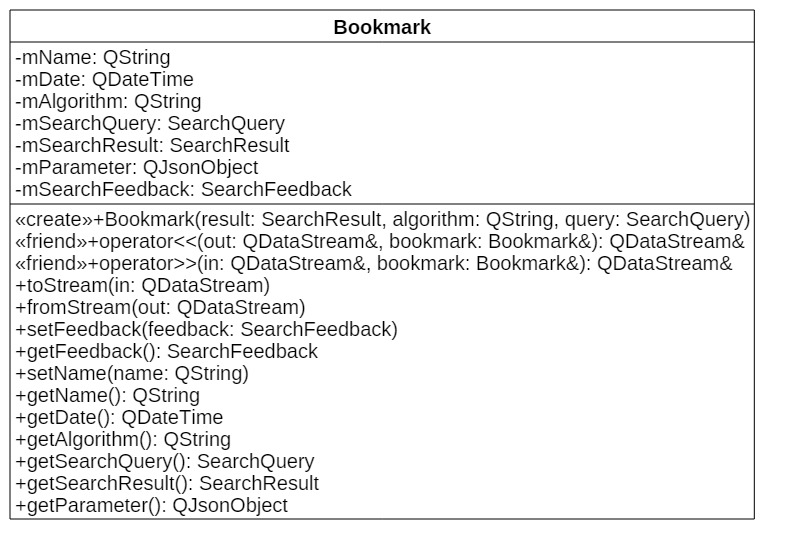
\includegraphics[scale=0.5]{img/Klassendiagramm/Klassen/Bookmark}
\label{fig:bookmark}
\end{figure}

Attribute
\begin{itemize}
\item\textit{private QString mName} Der Name dieses Bookmarks.
\item\textit{private QDateTime mDate} Die Zeit, zu der das Bookmark gespeichet wurde.
\item\textit{private QString mAlgorithm} Der Name des Algorithmus, der für diese Suche eingesetzt wurde.
\item\textit{private SearchQuery mSearchQuery} Die Suchanfrage dieser Suche.
\item\textit{private SearchResult mSearchResult} Das Suchergebnis dieser Suche.
\item\textit{private QJsonObject mParameter} Die für diese Suche gesetzten Parameter.
\item\textit{private SearchFeedback mSearchFeedback} Das vom Benutzer gesetzte Feedback.
\end{itemize}


Methoden
\begin{itemize}
\item \textit{public Bookmark(SearchResut result, QString algorithm, SearchQuery query} Erzeugt ein neues Bookmark.
\item \textit{public friend QDataStream\& operator<<(QDataStream\& out, Bookmark\& bookmark)} Speichert das Bookmark in einer Datei.
\item \textit{public friend QDataStream\& operator>>(QDataStream\& in, Bookmark\& bookmark)} Lädt das Bookmark aus einer Datei.
\item \textit{public void toStream(QDataStream in)} Speichert das Bookmark, durch den Aufruf von operator<<, in einer Datei.
\item \textit{public void fromStream(QDataStream out)} Lädt das Bookmark, durch den Aufruf von operator>>, aus einer Datei.
\item\textit{public void setFeedback(SearchFeedback feedback)} Speichert das Feedback im Bookmark.
\item\textit{public SearchFeedback getFeedback()} Gibt das Feedback zurück.
\item\textit{public void setName(QString name)} Setzt den Namen des Bookmarks.
\item\textit{public QString getName()} Gibt den Namen des Bookmarks zurück.
\item\textit{public QDateTime getDate()} Gibt die Zeit, zu der das Bookmark erstellt wurde, zurück.
\item\textit{public QString getAlgorithm()} Gibt den Namen des verwendeten Algorithmus zurück.
\item\textit{public SearchQuery getSearchQuery()} Gibt die Suchanfrage zurück.
\item\textit{public SearchResult getSearchResult()} Gibt das Suchergebnis zurück.
\item\textit{public QJsonObject getParameter()} Gibt die Parameter zurück.
\end{itemize}

\subsection*{BookmarkList}
Die BookmarkList hält eine Liste von Bookmarks und speichert die Bookmarks.

\begin{figure}[H]
\centering
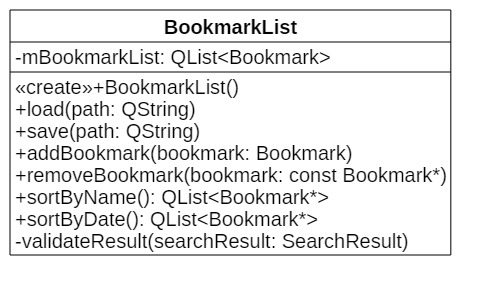
\includegraphics[scale=0.5]{img/Klassendiagramm/Klassen/BookmarkList}
\label{fig:bookmarkList}
\end{figure}

Attribute
\begin{itemize}
\item\textit{private QList<Bookmark> mBookmarkList} Eine Liste von Bookmarks.
\end{itemize}

Methoden
\begin{itemize}
\item \textit{public BookmarkList()} Erzeugt eine BookmarkList.
\item \textit{public void load(QString path)} Lädt die Bookmarks aus der Datei.
\item \textit{public void save(QString path)} Speichert die Bookmark Liste in der Datei mit dem übergebenen Pfad.
\item \textit{public void addBookmark(Bookmark bookmark)} Fügt ein Bookmark in die Liste hinzu.
\item \textit{public void removeBookmark(const Bookmark* bookmark)} Entfernt bookmark aus der BookmarkListe.
\item \textit{public QList<Bookmark*> sortByName()} Gibt die nach Namen sortierte Bookmarkliste zurück.
\item \textit{public QList<Bookmark*> sortByDate()} Gibt die nach Datum sortierte Bookmarkliste zurück.
\item \textit{private void validateResult(SearchResult searchResult)} Überprüft, ob das übergebene SearchResult gültig ist, also noch alle Datensätze und Medien vorhanden sind.
\end{itemize}

\subsection*{Dataset}
Ein Dataset hat einen Typ und enthält Medien von diesem Typ.

\begin{figure}[H]
\centering
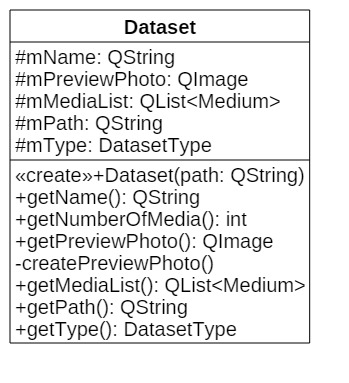
\includegraphics[scale=0.5]{img/Klassendiagramm/Klassen/Dataset}
\label{fig:dataset}
\end{figure}

Attribute
\begin{itemize}
\item\textit{protected QString mName} Der Name des Ordners.
\item\textit{protected QImage mPreviewPhoto} Das Vorschaubild dieses Datensatzes.
\item\textit{protected QList<Medium> mMediaList} Die Liste von Medium in diesem Datensatz.
\item\textit{protected QString mPath} Der Pfad dieses Datensatzes.
\item\textit{protected DatasetType mType} Der Typ dieses Datensatzes.
\end{itemize}

Methoden
\begin{itemize}
\item \textit{public Dataset(QString path)} Erzeugt einen Datensatz mit dem übergebenen Ordnerpfad.
\item \textit{public QString getName()} Gibt den Namen des Datensatzes (des Ordners) zurück.
\item \textit{public int getNumberOfMedia()} Gibt die Anzahl der Medien in der MediaList zurück.
\item \textit{public QImage getPreviewPhoto()} Gibt das Vorschaubild des Datensatzes zurück.
\item \textit{private void createPreviewPhoto()} Erstellt ein Vorschaubild aus den Medien.
\item \textit{public QList<Medium> getMediaList()} Gibt die Liste aller Medien zurück.
\item \textit{public QString getPath()} Gibt den absoluten Pfad des Datensatzes zurück.
\item \textit{public DatasetType getType()} Gibt den Typ des Datensatzes (und damit auch der Medien) zurück.
\end{itemize}

\subsection*{DatasetList}
Eine DatasetList hält eine Liste von Datensätzen und speichert sie.

\begin{figure}[H]
\centering
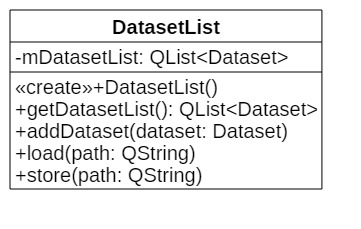
\includegraphics[scale=0.5]{img/Klassendiagramm/Klassen/DatasetList}
\label{fig:datasetList}
\end{figure}

Attribute
\begin{itemize}
\item\textit{private QList<Dataset> mDatasetList} Die Liste von Datensätze.
\end{itemize}

Methoden
\begin{itemize}
\item \textit{public DatasetList()} Erzeugt eine DatasetList.
\item \textit{public QList<Dataset> getDatasetList()} Gibt die Liste der Datensätze zurück.
\item \textit{public void addDataset(Dataset dataset)} Fügt den übergebenen Dataset der Liste hinzu.
\item \textit{public void load(QString path)} Lädt die Datensatzliste aus der Datei mit dem übergebenen Pfad.
\item \textit{public void store(QString path)} Speichert die Datensatzliste in der Datei mit dem übergebenen Pfad.
\end{itemize}

\subsection*{DatasetType}
Der Datensatztyp kann Photo, Video oder SingleFrameVideo sein.

\begin{figure}[H]
\centering
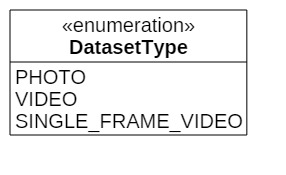
\includegraphics[scale=0.5]{img/Klassendiagramm/Klassen/DatasetType}
\label{fig:datasetType}
\end{figure}

\subsection*{Medium}
Ein Medium wird durch einen Pfad charakterisiert. Außerdem hat ein Medium eine Liste von Annotationen und den zugehörigen Index. Der Index ist bei Photos 0, in Videos gibt er an, in welchem Frame sich die Annotation befindet.

\begin{figure}[H]
\centering
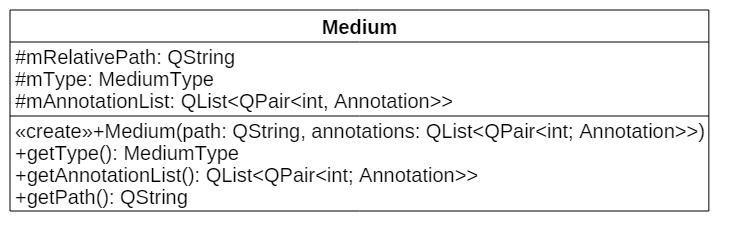
\includegraphics[scale=0.5]{img/Klassendiagramm/Klassen/Medium}
\label{fig:medium}
\end{figure}

Attribute
\begin{itemize}
\item\textit{protected QString mRelativePath} Der Pfad zu diesem Medium.
\item\textit{protected MediumType mType} Der Typ dieses Mediums.
\item\textit{protected QList<QPair<int, Annotation>> mAnnotationList} Die Liste von Annotationen für dieses Medium.
\end{itemize}

Methoden
\begin{itemize}
\item \textit{public Medium(QString path, QList<QPair<int, Annotation>> annotations)} Erzeugt ein Medium, das den übergebenen Pfad und die Annotationsliste hat.
\item \textit{public MediumType getType()} Gibt den Typ des Mediums zurück.
\item \textit{public QList<QPair<int, Annotation>>} Gibt die Liste der Annotationen zurück.
\end{itemize}

\subsection*{<<enumeration>> MediumType}
Der MediumType gibt den Typ des Mediums an: photo, video oder single frame video.

\begin{figure}[H]
\centering
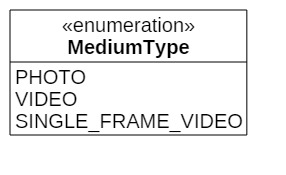
\includegraphics[scale=0.5]{img/Klassendiagramm/Klassen/MediumType}
\label{fig:mediumType}
\end{figure}

\subsection*{Photo : public Medium}
Ein Photo ist ein Bild, in dem Annotationen sein können.

\begin{figure}[H]
\centering
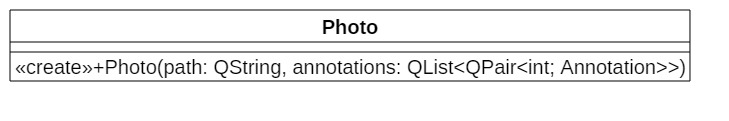
\includegraphics[scale=0.5]{img/Klassendiagramm/Klassen/Photo}
\label{fig:photo}
\end{figure}

Methoden
\begin{itemize}
\item \textit{public Photo(QString path)} Erzeugt ein Photo, mit dem übergebenen Pfad.
\end{itemize}

\subsection*{SingleFrameVideo : public Medium}
Ein SingelFrameVideo ist ein Video aus Einzelbildern.

\begin{figure}[H]
\centering
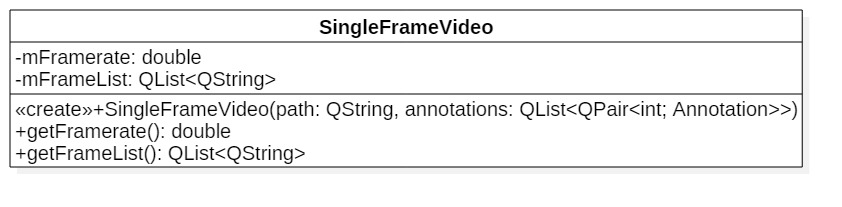
\includegraphics[scale=0.5]{img/Klassendiagramm/Klassen/SingleFrameVideo}
\label{fig:singleFrameVideo}
\end{figure}

Attribute
\begin{itemize}
\item\textit{private int mFramerate} Die Framerate dieses Videos.
\item\textit{private QList<QString> mFrameList} Die Liste von Frames dieses Videos.
\end{itemize}

Methoden
\begin{itemize}
\item \textit{public SingleFrameVideo(QString path)} Erzeugt ein SingleFrameVideo.
\item \textit{public int getFramerate()} Gibt die Framerate des Videos zurück.
\item \textit{public QList<QString> getFrameList()} Gibt die Liste der Frames zurück.
\end{itemize}

\subsection*{Video : public Medium}
Ein Video aus einer Videodatei.

\begin{figure}[H]
\centering
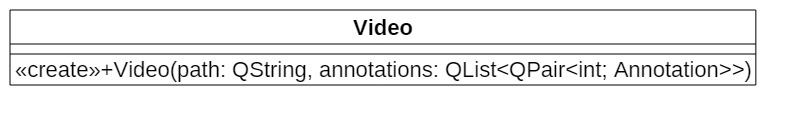
\includegraphics[scale=0.5]{img/Klassendiagramm/Klassen/Video}
\label{fig:video}
\end{figure}

Methoden
\begin{itemize}
\item \textit{public Video(QString path)} Erzeugt ein Video aus dem übergebenen Pfad.
\end{itemize}

\subsection*{<<interface>> Algorithm}
Die Algorithmen, die von CoBaB ausgeführt werden sollen, müssen mindestens diese Schnittstelle implementieren.

\begin{figure}[H]
\centering
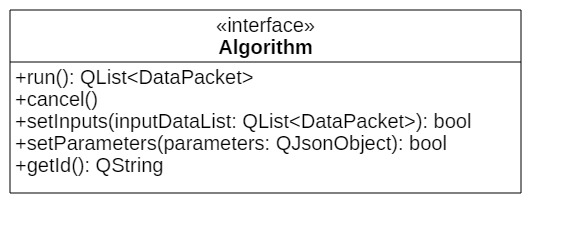
\includegraphics[scale=0.5]{img/Klassendiagramm/Klassen/Algorithm}
\label{fig:algorithm}
\end{figure}

Methoden
\begin{itemize}
\item\textit{public QList<DataPacket> run()} Startet den Algorithmus. Die Liste von DataPackets sind die Ergebnisse des Algorithmus.
\item\textit{public void cancel()} Bricht die Ausführung des Algorithmus ab.
\item\textit{public bool setInputs(QList<DataPacket> inputDataList)} Übergibt die benötigten Daten an den Algorithmus. Der Algorithmus gibt zurück, ob diese Liste seinen Eingabeparametern entspricht und es somit möglich ist, ihn zu starten.
\item\textit{public bool setParameters(QJsonObject parameters)} Übergibt die vom Benutzer festgelegten Parameterwerte an den Algorithmus. Der Algorithmus gibt zurück, ob diese Parameterdatei für ihn geeignet ist.
\item\textit{public QString getId()} Gibt eine für diesen Algorithmus eindeutige Identifikation zurück.
\end{itemize}

\subsection*{<<interface>> SearchAlgorithm : public Algorithm}
Die Implementierung dieser Schnittstelle ermöglicht CoBaB, genauere Angaben über den Algorithmus anzuzeigen.

\begin{figure}[H]
\centering
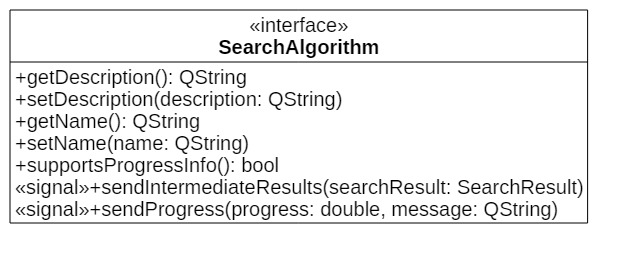
\includegraphics[scale=0.5]{img/Klassendiagramm/Klassen/SearchAlgorithm}
\label{fig:searchAlgorithm}
\end{figure}

Methoden
\begin{itemize}
\item\textit{public QString getDescription()} Gibt eine Beschreibung des Algorithmus zurück.
\item\textit{public void setDescription(QString description)} Setzt die Beschreibung des Algorithmus.
\item\textit{public QString getName()} Gibt den Namen des Algorithmus zurück.
\item\textit{public void setName(QString name)} Setzt den Namen des Algorithmus auf name.
\item\textit{public bool supportsProgressInfo()} Gibt zurück, ob der Algorithmus Fortschrittsinformationen senden kann.
\item\textit{public sendIntermediateResults(SearchResult searchResult)} Ist ein Signal, dass vom Algorithmus gesendet wird, wenn Zwischenergebnisse verfügbar sind.
\item\textit{public sendProgress(double progress, QString message)} Ist ein Signal, das den Fortschritt des Algorithmus sendet.
\end{itemize}

\subsection*{TestAlgorithm : public SearchAlgorithm}
Dieser Suchalgorithmus wird zu Testzwecken implementiert. Er generiert ein zufälliges SearchResult.

\begin{figure}[H]
\centering
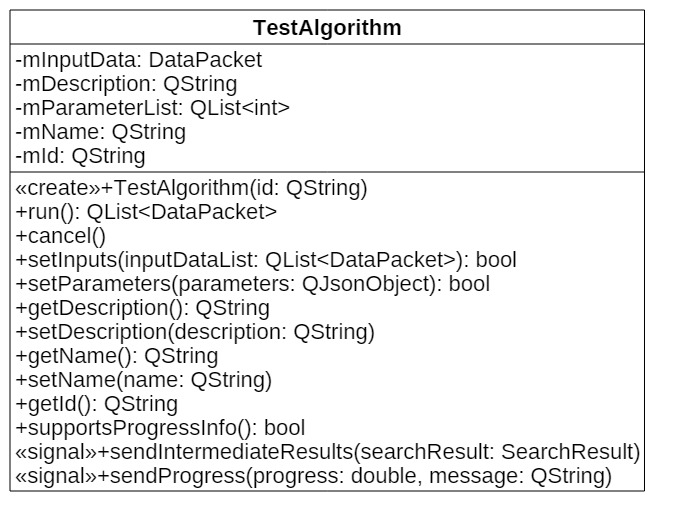
\includegraphics[scale=0.5]{img/Klassendiagramm/Klassen/TestAlgorithm}
\label{fig:testAlgorithm}
\end{figure}

Attribute
\begin{itemize}
\item\textit{private DataPacket mInputData} Die Eingabedaten für den Algorithmus.
\item\textit{private QString mDescription} Die Beschreibung für den Algorithmus.
\item\textit{private QList<int> mParameterList} Mögliche Einträge für die Parameterliste: randomSeed, sleep time interval.
\item\textit{private QString mName} Der Name des Algorithmus.
\item\textit{private QString mId} Die Id des Algorithmus.
\end{itemize}

Methoden
\begin{itemize}
\item\textit{public TestAlgorithm(QString id)} Erstellt einen neuen Test-Algorithmus.
\item\textit{public QList<DataPacket> run()} Startet den Algorithmus. Die Liste von DataPackets sind die Ergebnisse des Algorithmus.
\item\textit{public void cancel()} Bricht die Ausführung des Algorithmus ab.
\item\textit{public bool setInputs(QList<DataPacket> inputDataList)} Übergibt die benötigten Daten an den Algorithmus. Der Algorithmus gibt zurück, ob diese Liste seinen Eingabeparametern entspricht und es somit möglich ist, ihn zu starten.
\item\textit{public bool setParameters(QJsonObject parameters)} Übergibt die vom Benutzer festgelegten Parameterwerte an den Algorithmus. Der Algorithmus gibt zurück, ob diese Parameterdatei für ihn geeignet ist.
\item\textit{public QString getId()} Gibt eine für diesen Algorithmus eindeutige Identifikation zurück.
\item\textit{public QString getDescription()} Gibt eine Beschreibung des Algorithmus zurück.
\item\textit{public void setDescription(QString description)} Setzt die Beschreibung für den Algorithmus.
\item\textit{public QString getName()} Gibt den Namen des Algorithmus zurück.
\item\textit{public void setName(QString name)} Setzt den Namen des Algorithmus auf name.
\item\textit{public QString getId()} Gibt die Id des Algorithmus zurück.
\item\textit{public bool supportsProgressInfo()} Gibt zurück, ob der Algorithmus Fortschrittsinformationen senden kann.
\item\textit{public sendIntermediateResults(SearchResult searchResult)} Ist ein Signal, dass vom Algorithmus gesendet wird, wenn Zwischenergebnisse verfügbar sind.
\item\textit{public sendProgress(double progress, QString message)} Ist ein Signal, das den Fortschritt des Algorithmus sendet.
\end{itemize}

\subsection*{AlgorithmList}
Diese Liste verwaltet verfügbare Algorithmen.

\begin{figure}[H]
\centering
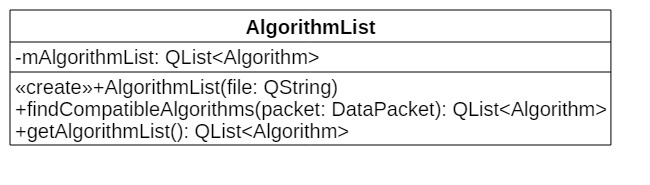
\includegraphics[scale=0.5]{img/Klassendiagramm/Klassen/AlgorithmList}
\label{fig:algorithmList}
\end{figure}

Attribute
\begin{itemize}
\item\textit{private QList<Algorithm> mAlgorithmList} Die Liste der verfügbaren Algorithmen.
\end{itemize}

Methoden
\begin{itemize}
\item\textit{public AlgorithmList(QString file)} Erzeugt eine Liste der verfügbaren Algorithmen.
\item\textit{public QList<Algorithm> findCompatibleAlgorithms(DataPacket packet)} Gibt das DataPacket als Eingabe an alle Algorithmen und gibt die Liste der Algorithmen zurück, die diese Eingabe akzeptiert haben.
\item\textit{public QList<Algorithm> getAlgorithmList()} Gibt die Liste der verfügbaren Algorithmen zurück.
\end{itemize}

\pagebreak

\subsection{View}

\begin{figure}[H]
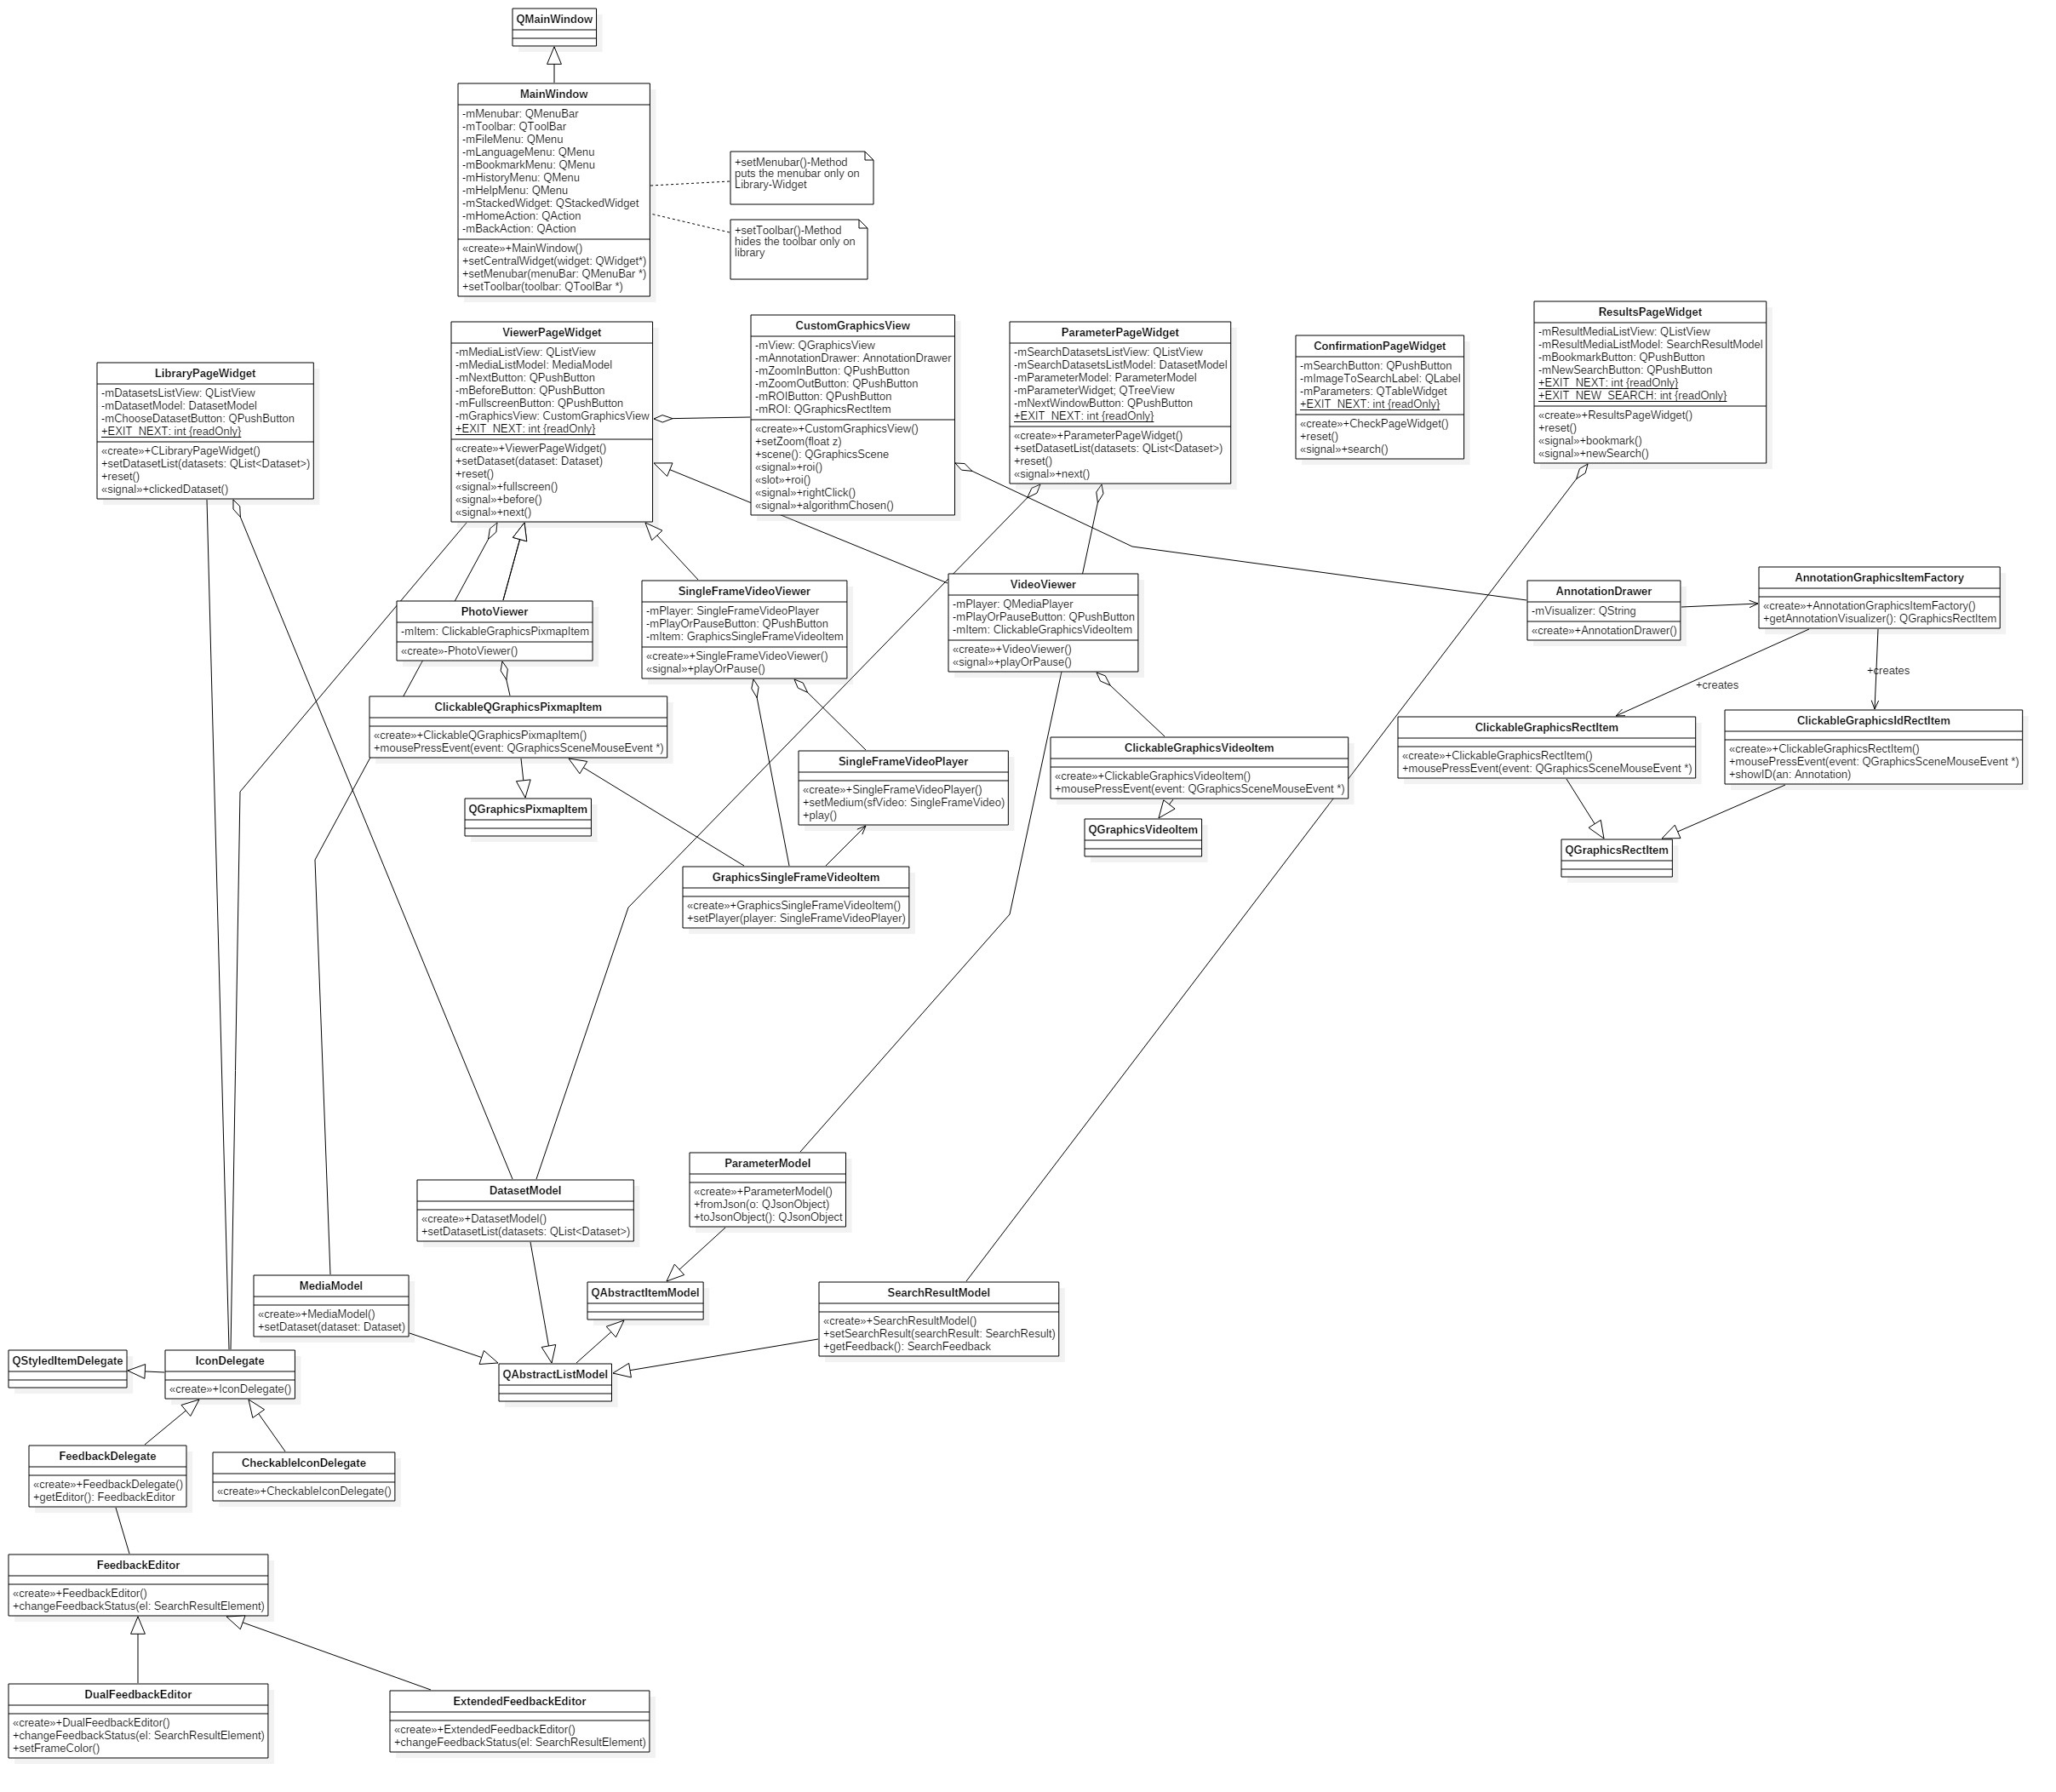
\includegraphics[width=1\linewidth]{img/Klassendiagramm/View}
\caption{View}
\label{fig:view}
\end{figure}


\subsection*{PageWidget}
Ein PageWidget ist ein QWidget, das als eine Seite der grafischen Oberfläche im MainWindow dem Benutzer angezeigt wird. Die abstrakte Klasse PageWidget bietet dem erbenden Widget, das momentan im MainWindow angezeigt wird, die Möglichkeit ein PageWidget auszusuchen, um es dem Benutzer als nächstes anzuzeigen, und diesem über den Stack des Navigators nötige Daten weiterzugeben.

\subsection*{<<enumeration>> PageType}
PageWidgets lassen sich beim Navigator mit einem PageType registrieren, welcher fortan zur Referenzierung dieses PageWidgets dient.

\subsection*{PageWidgetDispatcher}
Kapselt Signale, die zum verwenden des Stacks des Navigators und dem wechseln des PageWidgets nötig sind. (Ohne diese Kapselung stünden diese Signale den speziellen PageWidgets zur Verfügung)

\subsection*{MainWindow}
Die Klasse erbt von QMainWindow und stellt das Hauptfenster des Programms dar, auf dem die weiteren Seiten als Widgets angezeigt werden.

Attribute
\begin{itemize}
	\item\textit{private QMenuBar mMenubar}  
	\item\textit{private QToolbar toolbar}
	\item\textit{private QMenu mFileMenu}
	\item\textit{private QMenu mLanguageMenu}
	\item\textit{private QMenu mBookmarkMenu}
	\item\textit{private QMenu mHistoryMenu}
	\item\textit{private QMenu mHelpMenu}
	\item\textit{private QStackedWidget mStackedWidget}
	\item\textit{private QAction mHomeAction}
	\item\textit{private QAction mBackAction}
\end{itemize}

Methoden
\begin{itemize}
	\item\textit{public MainWindow()}
	\item\textit{public setCentralWidget(QWidget* widget)}
	\item\textit{public setMenubar(QMenuBar * menuBar)}
	\item\textit{public setToolbar(QToolBar * toolbar)}
\end{itemize}

\subsection*{LibraryPageWidget}
Das Widget, in dem alle Datensätze dargestellt werden. Man kann einen Datensatz für die Suche auswählen. Durch das ChooseDataSetButton kann man auch einen Datensatz wählen, der nicht in der Datenbank liegt. 

Attribute
\begin{itemize}
	\item\textit{private QListView mDatasetsListView}
	\item\textit{private CDatasetModel mDatasetModel}
	\item\textit{private QPushButton mChooseDatasetButton}
	\item\textit{public int EXIT\_NEXT}     
\end{itemize}

Methoden
\begin{itemize}
	\item\textit{public CLibraryPageWidget()}
	\item\textit{public setDatasetList(QList<Dataset>) datasets}
	\item\textit{public setMenubar(signal\_clicked\_Dataset())}
	\item\textit{public reset()}
\end{itemize}

\subsection*{ViewerPageWidget}
Diese Klasse erbt von QWidget und und bildet die Basis für die Widgets, die den Inhalt eines Datensatzes in Form von Photoalbum oder Videoplayer darstellen.

Attribute
\begin{itemize}
	\item\textit{private QListView mMediaListView}
	\item\textit{private CMediaModel mMediaListModel}
	\item\textit{private QPushButton mNextButton}
	\item\textit{private QPushButton MBeforeButton}
	\item\textit{private QPushButton mFullscreenButton}
	\item\textit{private CCustomGraphicsView mGraphicsView}
	\item\textit{public int EXIT\_NEXT}      
\end{itemize}

Methoden
\begin{itemize}
	\item\textit{public CViewerPageWidget()}
	\item\textit{public setDataset(Dataset dataset)}
	\item\textit{public signal\_Fullscreen()}
	\item\textit{public signal\_Before()}
	\item\textit{public signal\_Next()}
	\item\textit{public reset()}
\end{itemize}

\subsection*{PhotoViewer}
Erbt von ViewerPageWidget. Seine Funktion ist das Darstellen der Bilder, die in einem Datensatz enthalten sind.

Attribute
\begin{itemize}
	\item\textit{private CClickableGraphicsPixmapItem mItem}    
\end{itemize}

Methoden
\begin{itemize}
	\item\textit{public CPhotoViewer()}
\end{itemize}

\subsection*{ClickableQGraphicsPixmapItem}
Erbt von QGraphicsPixmapItem und stell das Bild dar, das bei CustomGraphicsView angezeigt wird und auf dem Annotationen gemacht werden können. Mit einem Rechtsklick kann man den Algorithmus für die Suche wählen.

Methoden
\begin{itemize}
	\item\textit{public CClickableQGraphicsPixmapItem()}
	\item\textit{public mousePressEvent(QGraphicsSceneMouseEvent *event)}
\end{itemize}

\subsection*{SingleFrameVideoViewer}
Erbt von ViewerPageWidget und seine Funktion ist das Darstellen der Videos in einem Datensatz, die in Form von EInzelbilder vorliegen.

Attribute
\begin{itemize}
	\item\textit{private CSingleFrameVideoPlayer mPlayer}
	\item\textit{private QPushButton mPlayOrPauseButton}
	\item\textit{private CGraphicsSingleFrameVideoItem mItem}    
\end{itemize}

Methoden
\begin{itemize}
	\item\textit{public CSingleFrameVideoViewer()}
	\item\textit{public signal\_PlayOrPause()}
\end{itemize}

\subsection*{CSingleFrameVideoPlayer} Eine Komponente, die das Video in Form von Einzelbildern in dem GraphicsView anzeigt.

Methoden
\begin{itemize}
	\item\textit{public CSingleFrameVideoPlayer()}
	\item\textit{public setMedium(SingleFrameVideo sfVideo)}
	\item\textit{public play()}
\end{itemize}

\subsection*{GraphicsSingleFrameVideoItem}
Erbt von ClickableQGraphicsPixmapItem und stellt mithilfe des SingleFrameVideoPlayers ein Video aus Einzeldateien, wobei man Annotationen machen und beim Rechtsklick den Algorithmus wählen kann.

Methoden
\begin{itemize}
	\item\textit{public CGraphicsSingleFrameVideoItem()}
	\item\textit{public setPlayer(CSingleFrameVideoPlayer player)}
\end{itemize}

\subsection*{VideoViewer}
Erbt von ViewerPageWidget. Seine Funktion ist das Darstellen und Abspielen der Videos, die in einem Datensatz enthalten sind.

Attribute
\begin{itemize}
	\item\textit{private QMediaPlayer mPlayer}
	\item\textit{private QPushButton mPlayOrPauseButton}
	\item\textit{private CClickableGraphicsVideoItem mItem}    
\end{itemize}

Methoden
\begin{itemize}
	\item\textit{public CVideoViewer()}
	\item\textit{public signal\_PlayOrPause()}
\end{itemize}

\subsection*{ClickableGraphicsVideoItem}


\subsection*{CustomGraphicsView}
Diese Klasse benutzt ein QGraphicsView um ein Bild darzustellen, AnnotationDrawer um die Annotationen die zum Bild gehören darzustellen und fügt die Möglichkeit hinzu, die Größe des Bildes durch die ZoomIn- und ZoomOutButton zu verändern, sowohl eine ROI(region of interest) zu zeichnen, nach der dann gesucht werden kann. Hier werden auch die Klicks der Benutzer abgefangen und die Menü mit den Algorithmen gezeigt.  

\subsection*{AnnotationDrawer}
Diese Klasse hat ein String, das bestimmt der Typ der Annotation und benutzt die AnnotationGraphicsItemFactory, um ein korrespondierendes ClickableGraphicsItem zu bekommen und dann zeigt dieses im CustomGraphicsView.
  
\subsection*{AnnotationGraphicsItemFactory}
Das ist eine Fabrik, die unterschiedliche ClickableGraphicsItems bildet, um man die Annotationen, abhängig von deren Typ, durch den AnnotationDrawer  darstellen zu können.

\subsection*{ClickableGraphicsIdRectItem}
Diese Klasse erbt von QGraphicsRectItem und fügt die Möglichkeit, auf dieses Item zu klicken hinzu, und zeigt die Id der Annotation.
 
\subsection*{ClickableGraphicsRectItem}
Diese Klasse erbt von QGraphicsRectItem und fügt die Möglichkeit, auf dieses Item zu klicken, hinzu.

\subsection*{ParameterPageWidget}
Das Widget, in dem die Parameter für den gewählten Suchalgorithmus gezeigt und bestimmt werden. Sowohl werden die Datensätze, in denen gesucht wird, bestimmt. Dann kann man zu ConfirmationPageWidget fortsetzen.

\subsection*{ConfirmationPageWidget}
Das Widget, in dem die Suchvorlage und alle Parameter angezeigt werden, sodass der Benutzer diese überprüfen kann. Mit dem SearchButton wird die Suche gestartet.

\subsection*{ResultsPageWidget}
Das Widget, wo die Ergebnisse der Suche erscheinen. Man kann die Suche speichern und bewerten. Nach der Bewertung kann erneut gesucht werden.

\subsection*{SearchResultModel}

\subsection*{ParameterModel}

\subsection*{DatasetModel}

\subsection*{MediaModel}

\subsection*{IconDelegate}
Diese Klasse erbt von QStyledItemDelegate und ist ein clickable IconDelegate, das aus einem Bild und darunter Text besteht. Diese nutzt man um die Datensätze in LibraryPageWidget, ViewerPageWidget darzustellen und herauszufinden welcher von denen selektiert ist.

\subsection*{CheckableIconDelegate}
Diese Klasse erbt von IconDelegate und eine Checkbox hinzufügt. Damit werden die Datensätze im ParameterPageWidget dargestellt und man bekommt die Information in welche von denen gesucht wird. 

\subsection*{FeedbackDelegate}
Die Klasse erbt von IconDelegate und kann ein FeedbackEditor benutzen, um Feedback zu bekommen. Man nutzt diese Klasse um die Resultate der Suche in ResultsPageWidget darzustellen, mit der Option Feedback zu bekommen. 

\subsection*{FeedbackEditor}
Diese Klasse stellt Feedback graphisch dar und bekommt die Wert des Feedbacks abhängig vom Typ des Feedbacks.

\subsection*{DualFeedbackEditor}

Stellt duales Feedback (positive, neutral, negative) dar.

\subsection*{ExtendedFeedbackEditor}
Stellt erweitertes Feedback (Werte von 1 bis 10) dar.

\pagebreak

\subsection{Controller}

\begin{figure}[H]
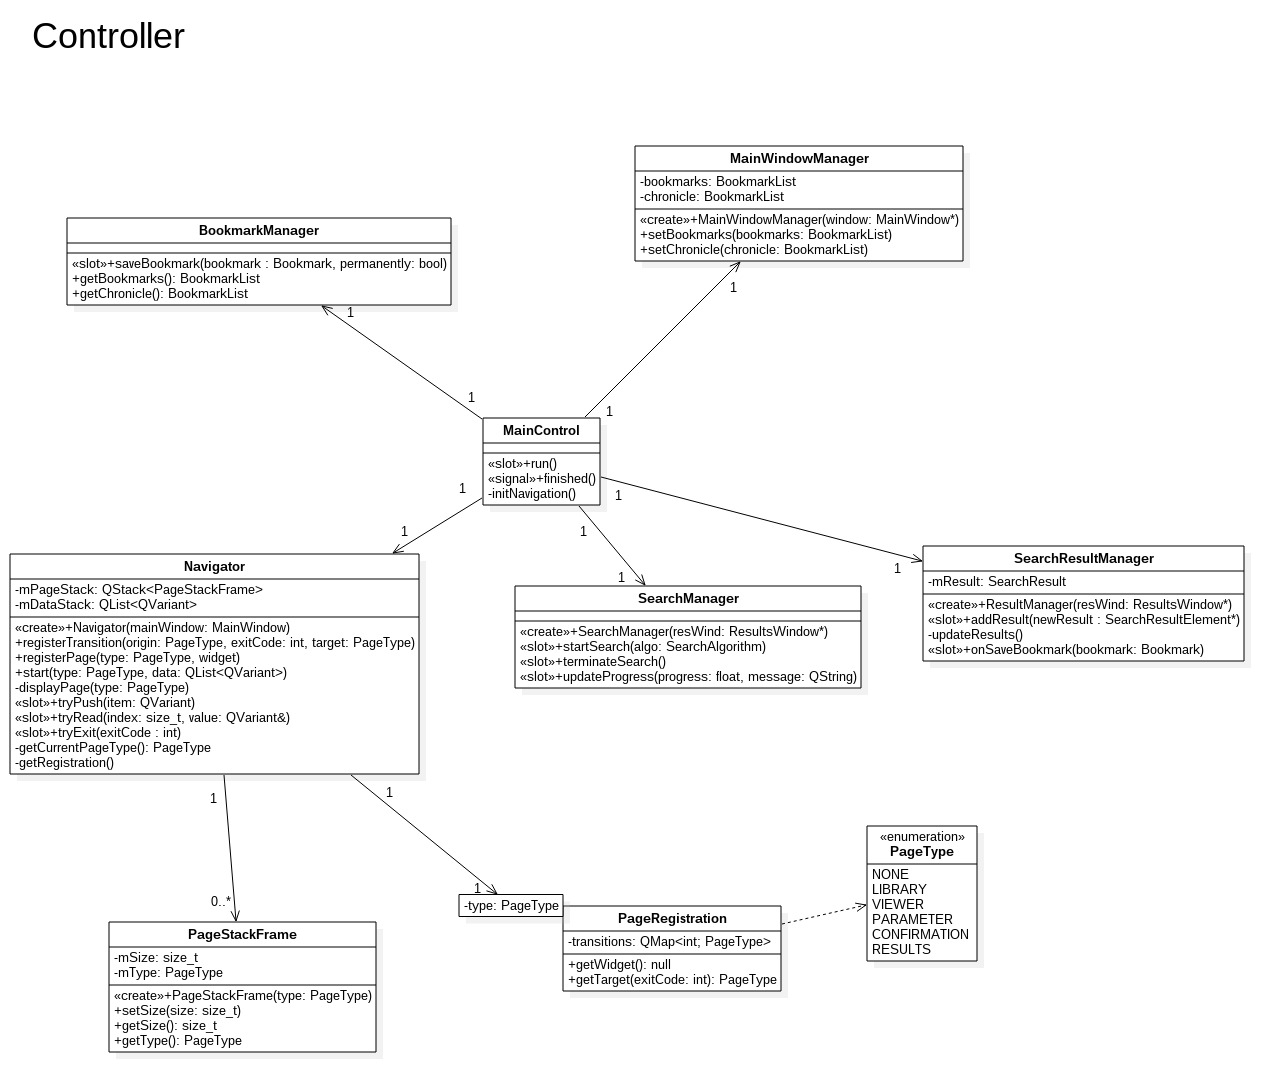
\includegraphics[width=1\linewidth]{img/Klassendiagramm/Controller}
\caption{Controller}
\label{fig:controller}
\end{figure}


\subsection*{MainControl}
MainControl ist der Einstiegspunkt des Programms und verwaltet die Manager-Klassen sowie den Navigator. Insbesondere erstellt MainControl die PageWidgets und registriert sie beim Navigator.
Da die Manager und der Navigator nicht direkt kommunizieren, verbindet MainControl ihre Signals und Slots.

\subsection*{Navigator}
Der Navigator ist in der Lage, das aktuell im MainWindow angezeigte PageWidget durch ein anderes zu ersetzen. Des weiteren ist der Navigator für den Austausch von Daten zwischen den PageWidgets verantwortlich.

\subsection*{SearchManager}
Der SearchManager startet einen Algorithmus in einem neuen Thread und leitet mögliche Informationen zum Fortschritt der Suche an das ResultsPageWidget weiter.

\subsection*{SearchResultManager}
Der SearchResultManager besitzt ein SearchResult und benachrichtigt das ResultsPageWidget über neue Suchergebnisse. Suchergebnisse können einzeln während der laufenden Suche hinzugefügt werden.

\subsection*{MainWindowManager}
Der MainWindowManager stellt die Bookmarks und Chronikeinträge dem MainWindow zur Verfügung und gibt bekannt, welches Bookmark im MainWindow zuletzt ausgewählt wurde.

\subsection*{BookmarkManager}
Der BookmarkManager besitzt 2 Listen für die Chronik und die vom Benutzer erstellten Bookmarks. Einträge für diese BookmarkLists werden über den BookmarkManager hinzugefügt und abgefragt.
